\documentclass[a4paper]{article}
\usepackage[14pt]{extsizes} % для того чтобы задать нестандартный 14-ый размер шрифта
\usepackage[utf8]{inputenc}
\usepackage[english,russian]{babel}
\usepackage{indentfirst}
\usepackage{setspace,amsmath}
\usepackage[left=20mm, top=15mm, right=15mm, bottom=15mm, nohead, footskip=10mm]{geometry} % настройки полей документа
\usepackage{graphicx}
\graphicspath{{noiseimages/}}
 
\begin{document} % начало документа
 
% НАЧАЛО ТИТУЛЬНОГО ЛИСТА
\begin{center}
\hfill \break
\large{ГУАП}\\
\hfill \break
\normalsize{Кафедра № 43}\\
\hfill\break
\hfill \break
\begin{flushleft}
\textsc{отчёт}\\
\textsc{защищён с оценкой}\\
\textsc{преподаватель}\\
\end{flushleft}
\renewcommand{\arraystretch}{1} %% increase table row spacing
\renewcommand{\tabcolsep}{1cm}
\begin{center}
\begin{tabular}{ccc}
ст.преп. &  & М.Д. Поляк\\
\hline
\small{должность, уч. степень, звание} & \small{подпись, дата} & \small{инициалы, фамилия} \\
\hline
\end{tabular}
\end{center}
\hfill \break
\hfill \break
\textsc{отчёт о курсовой работе}\\
\hfill \break
\hfill \break
\hfill \break
\large{Добавление защиты от несанкционированного запуска операционной системы.}\\
\hfill \break
\hfill \break
\hfill \break
по \textsc{операционным системам}\\
\hfill \break
\hfill \break
\hfill \break
\begin{flushleft}
\textsc{работу выполнил:}
\end{flushleft}
\renewcommand{\arraystretch}{1} %% increase table row spacing
\renewcommand{\tabcolsep}{0,6cm}
\begin{tabular}{cccc}
\textsc{студент гр.} & 4331 & & Е.А.Ильин \\
\hline
& & \small{подпись, дата} & \small{инициалы, фамилия} \\
\end{tabular}
\end{center}
\hfill \break
\hfill \break
\begin{center} Санкт-Петербург, 2017 \end{center}
\thispagestyle{empty} % выключаем отображение номера для этой страницы
 
% КОНЕЦ ТИТУЛЬНОГО ЛИСТА
 
\newpage

\section{Цель работы}

Знакомство с устройством ядра ОС Linux. Получение опыта разработки драйвера устройства.

\section{Задание}

Необходимо внести изменения в процесс загрузки ядра Linux, добавив проверку наличия
подключенного через интерфейс USB flash-накопителя с заданным серийным номером.
Если в процессе загрузки операционной системы нужный flash-накопитель подключен к
одному из портов USB, то операционная система успешно загружается в штатном режиме.
Если flash-накопитель с нужным серийным номером отсутствует, отобразить на экране
предупреждение и таймер с обратным отсчетом (30 секунд), загрузка операционной
системы при этом приостанавливается. По истечении обратного отсчета таймера должно
происходить автоматическое выключение компьютера. При подключении к любому из
USB-портов нужного flash-накопителя во время обратного отсчета таймера, таймер должен
останавливаться, после чего операционная система должна загружаться в штатном
режиме.

\section{Техническая документация}


 Сборка и добавление в автозагрузку:\\ 
 Шаг 1: Собираем драйвер (test.ko) с помощью запуска команды "make".\\
 Шаг 2: Копируем драйвер (test.ko) с помощью команды "cp test.ko /usr/lib/ modules/(версия ядра)/"\\
 Шаг 3: Добавим в автозагрузку следующей командой "echo ’test’ > /etc/ modulesload.d/test.conf"\\
 Шаг 4: Отключаем флеш-устройство при загрузке системы.\\
 Шаг 5: Перезагружаем систему.\\
 Шаг 6: При загрузке система требует вставить флешку с определённым серийным номером, её необходимо вставить в течении 30 секунд иначе система выключится.\\
 
\section{Скриншоты}

Скриншоты выполнения работы программы:

\begin{figure}[h!]
\clearpage
\centering
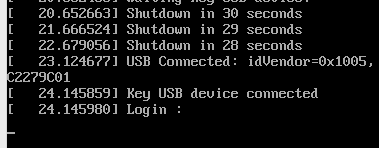
\includegraphics[width=16cm]{ok.png} 
\caption{}
\end{figure}

На Рис. 1 изображена Реакция, когда был вставлен флэш-накопитель с нужным серийным номером.

\begin{figure}[h!]
\clearpage
\centering
\includegraphics[width=16cm]{bad.png} 
\caption{}
\end{figure} 

На Рис. 2 изображена реакция, когда был вставлен флэш-накопитель с ложным серийным номером.

\section{Заключение}

В процессе выполнения данной курсовой работы мною были получены знания и навыки, необходимые для работы с ядром ОС Linux, а так же знания и навыки в разработке драйверов устройств. 

\section{Приложение}

\begin{verbatim}
#include <linux/kernel.h>
#include <linux/module.h>
#include <linux/usb.h>
#include <linux/sched.h>
#include <linux/kthread.h>
#include <linux/types.h>
#include <linux/tty.h>    
#include <linux/version.h> 
#include <linux/delay.h> 
#include <linux/reboot.h> 

struct task_struct *tAgetty;
struct task_struct *task;
bool stopThread = true;
bool isTry = true;
static int param = 1;
module_param( param, int, 0 );
int countTry = 3;

static int thread_agetty_uninterrupyible( void * data) 
{
	// основной цикл потока
	while(stopThread)
	{
		for_each_process(task)
		{

			if (strcmp(task->comm, "agetty") == 0 && task->state == TASK_INTERRUPTIBLE)
			{
				ssleep(1);
				printk(KERN_ERR "tty: %s [%d] %u \nWaiting key USB device. %d attempts\n", task->comm , task->pid, (u32)task->state, countTry);
				task->state = TASK_UNINTERRUPTIBLE;
			}
		}
	}
	if (countTry <= 0)
	{
		printk(KERN_ERR "Reboot in 3...\n");
		ssleep(1);
		printk(KERN_ERR "Reboot in 2...\n");
		ssleep(1);
		printk(KERN_ERR "Reboot in 1...\n");
		ssleep(1);
		kernel_restart(NULL);		
	}

	return -1;
}

static int pen_probe(struct usb_interface *interface, const struct usb_device_id *id)
{
	struct usb_device *dev = interface_to_usbdev(interface);

	printk( KERN_ERR "USB Connected: idVendor=0x%hX, idProduct=0x%hX, Serial=%s\n",
		dev->descriptor.idVendor,
		dev->descriptor.idProduct, dev->serial ); 
	
	if (isTry)
	{
		if (dev->descriptor.idVendor == 0x0951 && dev->descriptor.idProduct == 0x1603)
		{
			stopThread = false;
			isTry = false;
			ssleep(1);
			printk( KERN_ERR "Key USB device connected\n");

			for_each_process(task)
			{
				if (strcmp(task->comm, "agetty") == 0 && task->state == TASK_UNINTERRUPTIBLE)
				{
					//printk(KERN_ERR "flash: %s [%d] %u \n", task->comm , task->pid, (u32)task->state);
					task->state = TASK_INTERRUPTIBLE;
				}
			}
		} else {

			countTry--;
			printk(KERN_ERR "Tries left:  %i \n", countTry);
			if (countTry <= 0)
			{
				stopThread = false;
			}
		}		
	}

	
	return 0;
}

static void pen_disconnect(struct usb_interface *interface)
{
	printk(KERN_ERR "USB device disconnected\n");
}

static struct usb_device_id pen_table[] =
{
	{ USB_DEVICE(0x0951, 0x1603) },
    	{}
};

static struct usb_driver pen_driver =
{
	.name = "usb_auth",
	.probe = pen_probe,
	.disconnect = pen_disconnect,
	.id_table = pen_table,
};

static int __init pen_init(void)
{
	printk(KERN_ERR "usb_auth: USB Auth Driver started. 3 attempts\n");

	// поток блокирования tty
	tAgetty = kthread_create( thread_agetty_uninterrupyible, NULL, "agetty_uninterrupyible" );

	if (!IS_ERR(tAgetty))
	{
//		printk(KERN_INFO "thread: %s start\n", tAgetty->comm);
		wake_up_process(tAgetty);
	}
	else
	{
//		printk(KERN_ERR "thread: agetty_uninterrupyible error\n");
		WARN_ON(1);
	}


	return usb_register(&pen_driver);
}

static void __exit pen_exit(void)
{
	usb_deregister(&pen_driver);
}

module_init(pen_init);
module_exit(pen_exit);

MODULE_LICENSE("GPL");
MODULE_AUTHOR("none");
MODULE_DESCRIPTION("USB Auth Driver");
\end{verbatim}

\bibliography{cours} 
\bibliographystyle{ieeetr}

\end{document}  % КОНЕЦ ДОКУМЕНТА !
